\chapter{基于注意力机制的多股票关系模型}
\label{cha: msra}
为了解决新闻驱动的股票预测问题,我们把它转化为针对某一方面的情感分析问题(Aspect-Category Sentiment Analysis)。我们提出了基于注意力机制的多股票关系(Multi-Stock Relation Model using Attention Mechanism,MSRMAM)模型,该模型包括情感分析模块和股票关系模块。在本章中,我们首先给出问题的形式化描述,并简要介绍模型的结构,然后分别介绍情感分析模块和股票关系模块。
\begin{figure}[H] % use float package if you want it here
    \centering
    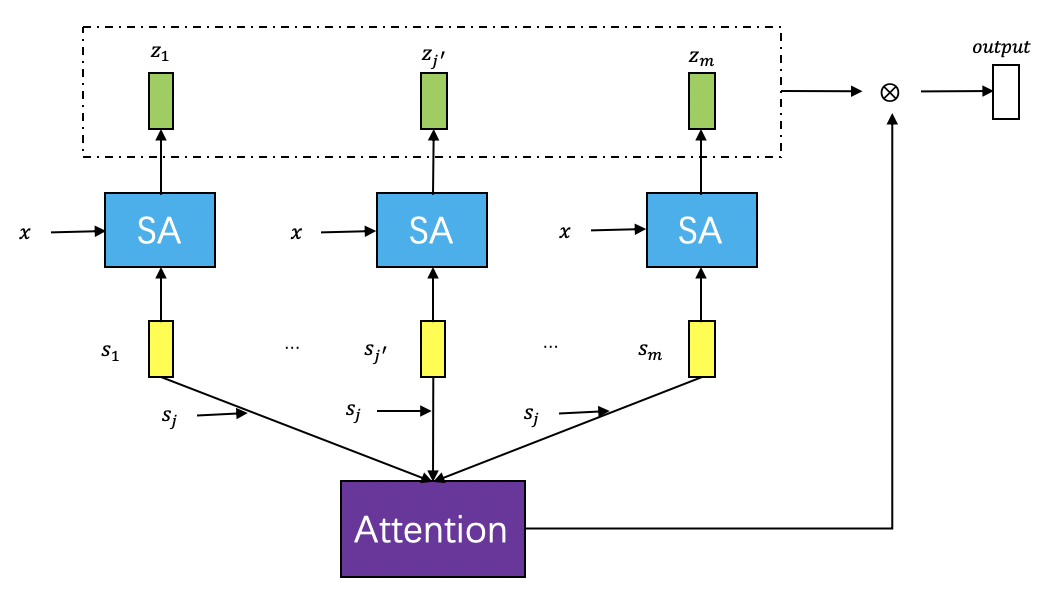
\includegraphics[width =0.8\linewidth]{figures/stock-relation.png}
    \caption{基于注意力机制的多股票关系模型结构}
    \label{fig: modelstructure}
\end{figure}

\section{问题描述}

问题的输入包括一支股票$s$以及一条与这支股票相关的新闻$w$,其中$w=\{w_1, w_2...w_n\}$,$n$是新闻句子的长度。句子相应的词向量表示是$x =\{x_1, x_2...x_n\}$。我们使用股票向量$s_j$来表示第$j$支股票,其中$j = 1, 2...m$,$m$是所有股票的数量。问题的输出是股票价格在下一个时间段内将会如何变化$y\in \{+1, 0, -1\}$,其中,$+ 1$表示股票的价格将会在下一天、周、月之后上涨,$- 1$表示股票的价格将会在下一天、周、月之后下跌,其它的为$0$。$C = 3$是输出标签的数量。比如,“微软收购诺基亚的手机部门”这一新闻对微软来说是积极的,将会使微软(MSFT)的股票价格上涨;对诺基亚来说是消极的,将会使诺基亚(NOK)的股票价格下跌。
\section{模型结构}
图~\ref{fig: modelstructure}展示了模型的基本结构。我们使用情感分析模块提取与股票$j$相关的新闻$w$的情感表示;使用点积注意力机制来学习股票之间的相关关系。所有股票的情感表示的加权和被用来作为输入的最终表示。最后使用带有softmax激活函数的全连接得到输出结果。
\section{股票向量}
在预测股票价格变化时,股票相关的信息有着重要的作用。同一条新闻,对不同的股票可能会产生完全不同的影响。为了更好地利用股票相关的信息,我们提出了股票向量的概念。我们为全部的股票构建一个词表,并为每支股票创建一个向量表示。向量$s_i\in R ^ {d_s}$表示的是第$i$支股票的向量表示,其中$d_s$表示的是股票向量的维度。$S\in R ^ {d_s\times | S |}$由全部的股票向量组成。据我们所知,这是第一次提出股票向量的概念。
\section{情感分析模块}

\begin{figure}[ht]
    \centering
    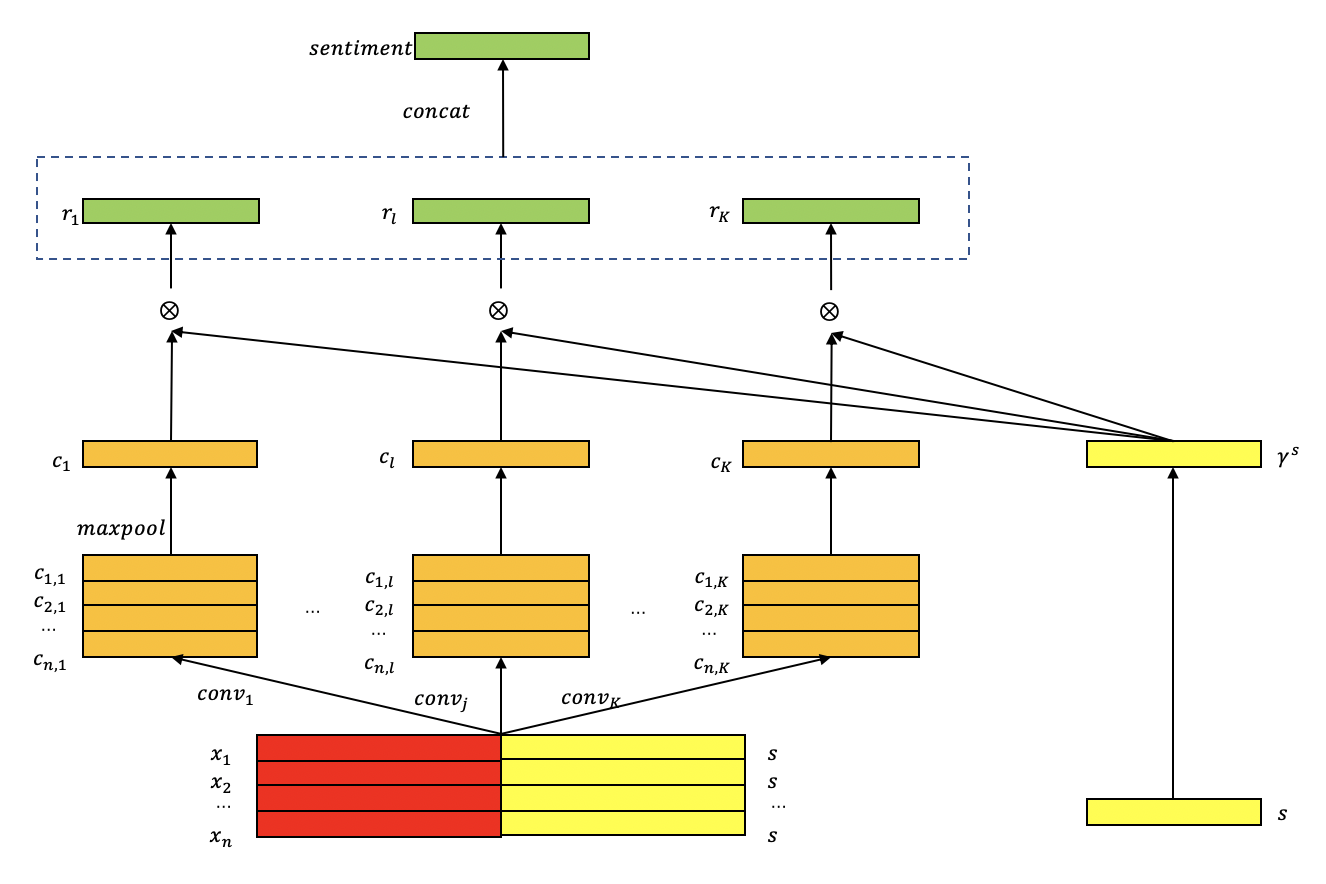
\includegraphics[width= \linewidth]{sentiment-analysis.png}
    \caption{情感分析模块}
    \label{fig: sentiment}
\end{figure}

如图~\ref{fig: sentiment}所示,情感分析模块使用了带有股票系数的多尺度卷积。

\subsection{多尺度卷积}
我们利用多尺度卷积来处理词向量。自然语言处理中常使用LSTM来处理句子序列,LSTM沿着时间维度,逐次计算下一个时间的隐层状态,从而将变长的序列转化为了定长输出。然后,因为LSTM的时序性,使得它难以并行化。CNN最初用于图片分类,CNN通过局部感受野,能够提取局部的特征。多层CNN在图像相关领域取得了非常优秀的表现,然而,CNN在自然语言处理领域一直没有得到很好的应用。直到TextCNN\cite{kim2014convolutional}提出,CNN才开始在自然语言处理中有所表现。相比于LSTM,CNN使用卷积核处理序列中局部的序列,更易于并行化。为了更好地结合股票相关信息,我们将句子的词向量$x_i$与股票向量$s$沿最后一个维度拼接起来。
\begin{equation}
    u_i = concat([x_i, s],axis=-1)
\end{equation}
卷积可以提取局部的特征,一个卷积核大小为$k$的卷积操作,可以将相邻的$k$个单词的信息结合起来,相当于得到了长度为$k$的短语的特征。多尺度卷积使用了多个不同卷积核大小的卷积层,这样,可以提取不同长度的短语的特征。
\begin{equation}
    c_{i, l} = relu(u_{i: i+k_l}*W_l+b_l)
\end{equation}
其中,$W_l$和$b_l$是第$l$个卷积的参数,$k_l$是第$l$个卷积的卷积核大小, $l = 1, 2...K$,$K$是不同尺度卷积的数量。$relu$激活函数的定义如下。
\begin{equation}
    relu(x) =\begin{cases}
        x & x > 0 \\
        0 & x\le 0
    \end{cases}
\end{equation}
最大池化(Max-pooling)层选取值最高的特征,其思想在于把最重要的特征选取出来。同时,max-pooling层可以将变长的序列转化为固定的长度,方便后续的处理。
\begin{equation}
    c_l = max(c_{1, l}, c_{2, l}...c{n, l})
\end{equation}
之前的研究表明\cite{kim2014convolutional},多层卷积神经网络CNN在自然语言处理中表现并不突出,却使得模型更深,更加难以训练,因此,我们这里只使用了单层卷积,并未使用多层的CNN结构。
\subsection{股票系数}
不同的股票具有不同的特性,有些股票更倾向于上涨,有些股票更倾向于下跌。为了更好地利用股票的特性,我们计算股票系数,它反映了股票的信息。
\begin{equation}
    \gamma ^ s = tanh(W_sx ^ s+b_s)
\end{equation}
其中, $W_s$和$b_s$是需要学习的参数。$tanh$函数的定义如下:
\begin{equation}
    tanh(x) =\frac{e ^ x-e ^ {-x}}{e ^ x+e ^ {-x}}
\end{equation}
我们用按元素的乘法将股票系数和句子表示结合起来。这里使用按元素的乘法,股票系数起到了对原有特征进行调整的作用,从而使得本来的特征带有了股票的相关信息。这里,股票系数可以看作是一个控制门,由$tanh$得到的激活值的取值范围在负无穷到正无穷之间,股票系数与前面得到的情感特征相乘,可以调整情感特征的值的幅度,从而引入了股票的相关信息。
\begin{equation}
    r_l = c_l\otimes \gamma ^ s
\end{equation}
全部卷积的结果沿最后一个维度拼接起来,得到句子的最终表示。
\begin{equation}
    r = concat([r_1, r_2...r_K],axis=-1)
\end{equation}
\section{股票关系模块}

股票公司之间的竞争、合作、上游、下游关系,可能会影响股票价格的变动。比如,“亚马逊向中国及其他七个国家的卖家提供贷款”对亚马逊(AMZN)来说是一条积极的新闻,它将会使得亚马逊的股票价格上升;同时,它也会对亚马逊在中国的竞争者阿里巴巴(BABA)造成消极的影响,使得其股票价格下跌。

\begin{figure}[H] % use float package if you want it here
	\centering
	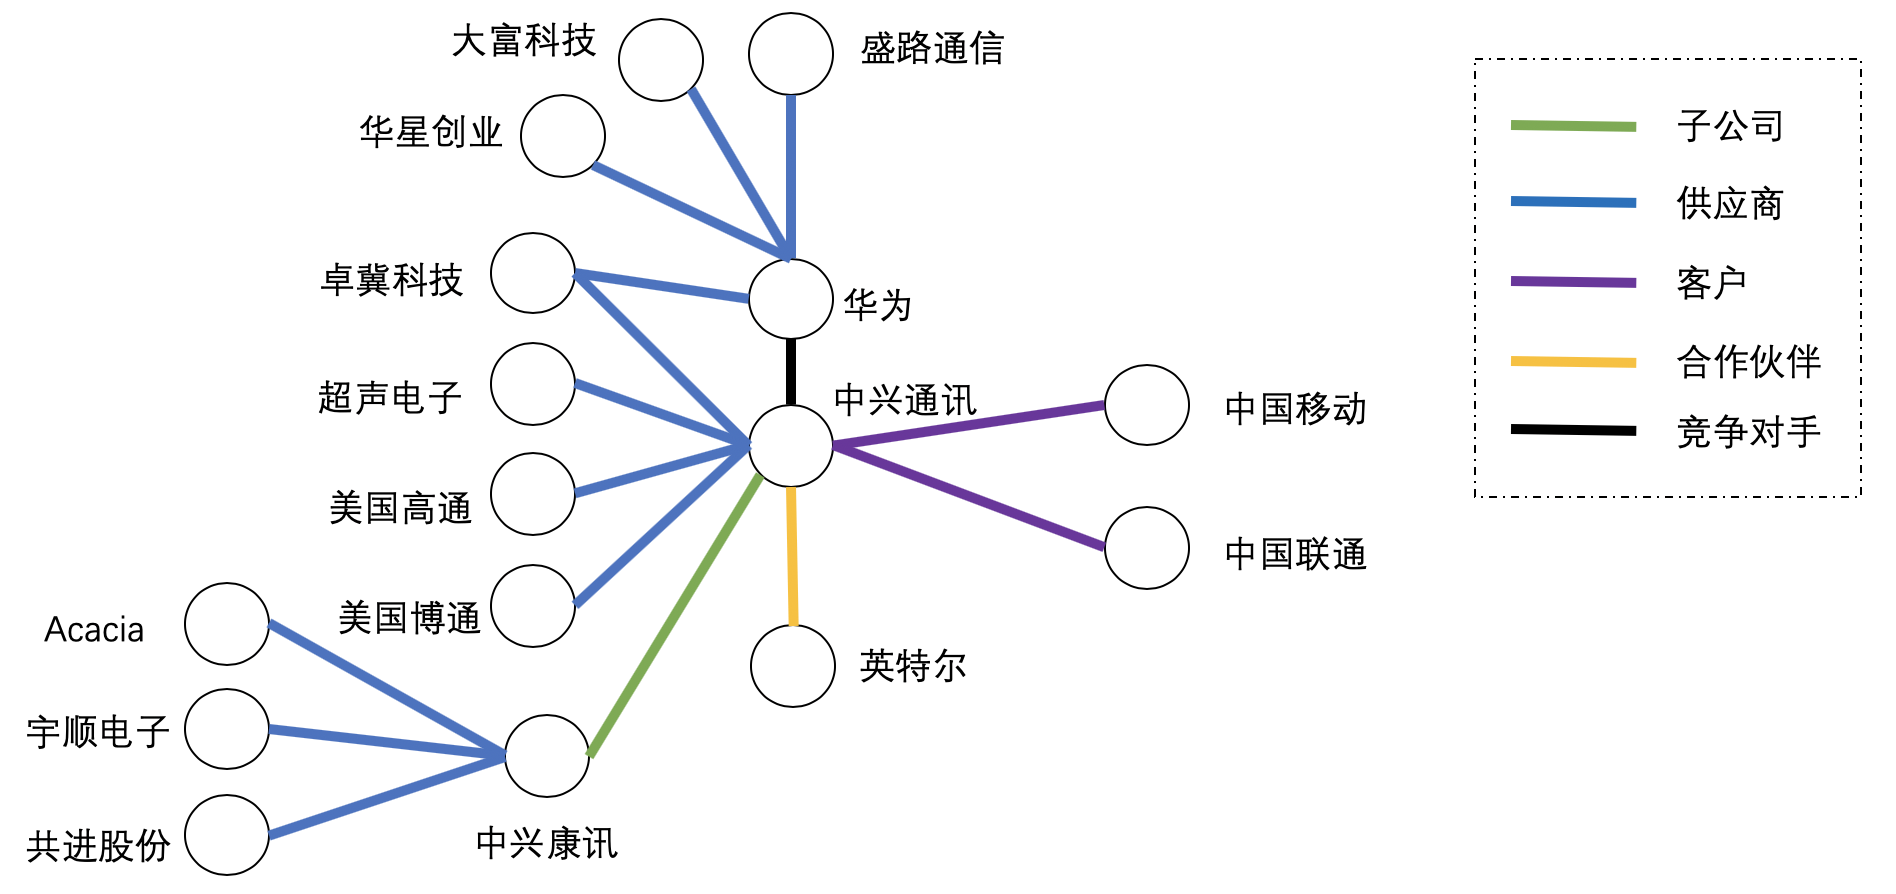
\includegraphics[width =\linewidth]{stockrelation.png}
	\caption{股票关系示例}
	\label{fig:stockrelationexample}
\end{figure}

图\ref{fig:stockrelationexample}显示了一些股票之间的相互关系的例子。我们使用点积attention来学习股票之间的相互关系。为了简便,我们使用下面的公式来表示情感分析模块的输出。
\begin{equation}
    z_{j'}=SA(x,s_{j'})
\end{equation}
其中,$j'=1, 2...m$是股票的序号。Attention的权重通过下面的公式求得,权重的大小与股票之间的点积相似度呈正相关。我们把所有股票的情感表示的加权和作为输入的最终表示。
\begin{equation}
    \begin{aligned}
        \alpha_{j'}&=\frac{s^T_{j}s_{j'}}{\sum_{j'=1}^{m}s^T_{j}s_{j'}}
        z &= \sum_{j'=1}^{m} \alpha_{j'}z_{j'}
    \end{aligned}
\end{equation}
\section{目标函数}

最后,由全连接层和softmax激活函数得到最终的预测结果。

\begin{equation}
    \hat{y}=softmax(Wz+b)
\end{equation}
其中,$W$和$b$是需要学习的参数。目标函数是实际值$y$和预测值$\hat{y}$之间的交叉熵。
\begin{equation}
    loss=\sum_{p} ^ {N}\sum_{c} ^ {C}\hat{y_{i, j}}log(y_{i, j})
\end{equation}
其中,$p$是样本序号,$c$是类别序号,$N$是样本数量,$C$是类别数量。
